\documentclass[11pt,a4paper]{ivoa}
\input tthdefs
\input gitmeta
\usepackage{todonotes}
\usepackage{textcomp}

\newcommand{\xsamsref}[1]{\textsuperscript{\ref{#1}}}

\lstloadlanguages{SQL,XML}
\lstset{flexiblecolumns=true,numberstyle=\small,showstringspaces=False,
  identifierstyle=\texttt}

\definecolor{lightgray}{rgb}{0.8,0.8,0.8}
\def\rowsep{\noalign{\vspace{2pt}}}

% since we don't do a lot of UCDs here and XSAMS references share a lot
% of the typesetting issues of UCDs, we'll re-use the ucd macro for now
% for them:
\let\xsref=\ucd

\newenvironment{xsamsbridge}
  {\begin{list}{}{\setlength\labelwidth{15em}%
    \setlength\labelsep{1em}%
    \setlength\leftmargin{5em}%
    }}
  {\end{list}}

\title{LineTAP: IVOA Relational Model for Spectral Lines}

% see ivoatexDoc for what group names to use here
\ivoagroup{DAL}

\author{Castro Neves, M.}
\author{Moreau, N.}
\author{Demleitner, M.}

\editor{Margarida Castro Neves, Nicolas Moreau}


\previousversion{This is the first public release}

\begin{document}
\begin{abstract}

This document proposes a relational schema to describe spectral line
transitions that can be queried using the TAP protocol. Its purpose is
to derive from the VAMDC data model a simplified way to query
spectral line databases from VO applications. The underlying model is
rooted in the widely-deployed VAMDC, and the intent is that at least the
atomic and molecular data from VAMDC can easily be re-published using
LineTAP.


\end{abstract}


%\section*{Acknowledgments}


\section*{Conformance-related definitions}

The words ``MUST'', ``SHALL'', ``SHOULD'', ``MAY'', ``RECOMMENDED'', and
``OPTIONAL'' (in upper or lower case) used in this document are to be
interpreted as described in IETF standard RFC2119 \citep{std:RFC2119}.

The \emph{Virtual Observatory (VO)} is a
general term for a collection of federated resources that can be used
to conduct astronomical research, education, and outreach.
The \href{http://www.ivoa.net}{International
Virtual Observatory Alliance (IVOA)} is a global
collaboration of separately funded projects to develop standards and
infrastructure that enable VO applications.


\section{Introduction}

The Simple Line Access Protocol SLAP \citep{2010ivoa.specQ1209O}
currently is the VO
recommendation for querying spectral line collections.
It is based on the Simple Spectral Line Data
Model SSLDM \citep{2010ivoa.spec.1209O}, which defines the underlying
data model.
As  in SSLDM, a \emph{spectral line} in this document is considered to
be the result of a (radiative) transition between two energy levels.

More than ten years after the protocol's definition, there are still
very few SLAP services registred in the VO.
On the other hand, the Virtual Atomic and Molecular Data Center
VAMDC \citep{atoms8040076} offers a great amount of spectral line
data.  Making this data available to VO clients without major extra
tooling is certainly desirable.

While the query part of VAMDC clearly betrays its origins in VO
standards and thus might readily be integrated into the VO protocol
stack, the service output comes in a very comprehensive derivative of
the XML Schema for Atomic, Molecular and Solid Data XSAMS
\citep{XSAMS:Docs}; in particular, its tree-like nature complicates
casual use.  In addition, many interesting use cases can already be
satisfied with a simple relational mapping of XSAMS.

This document proposes LineTAP, a simple way to access spectral line
data through a VO service employing such a simplified relational
mapping.  The resulting table schema is presented in
section~\ref{sect:quantities}, while the mapping between our columns and the
VAMDC-XSAMS Data Model is given in section~\ref{sect:mapping}.

When accessed using the Table Access Protocol TAP
\citep{2019ivoa.spec.0927D}, the table can be queried using the
expressive SQL-derived query language ADQL, while query results are
available in the VOTable format, easily readable by VO client
applications.  Line databases accessible in this way can be registered
in the VO Registry.  The detailed rules for this registration, and
recommendations for how to discover LineTAP services, are given in
section~\ref{sect:regmatters}.

\subsection{Role within the VO Architecture}

\begin{figure}
\centering

% As of ivoatex 1.2, the architecture diagram is generated by ivoatex in
% SVG; copy ivoatex/archdiag-full.xml to role_diagram.xml and throw out
% all lines not relevant to your standard.
% Notes don't generally need this.  If you don't copy role_diagram.xml,
% you must remove role_diagram.pdf from SOURCES in the Makefile.

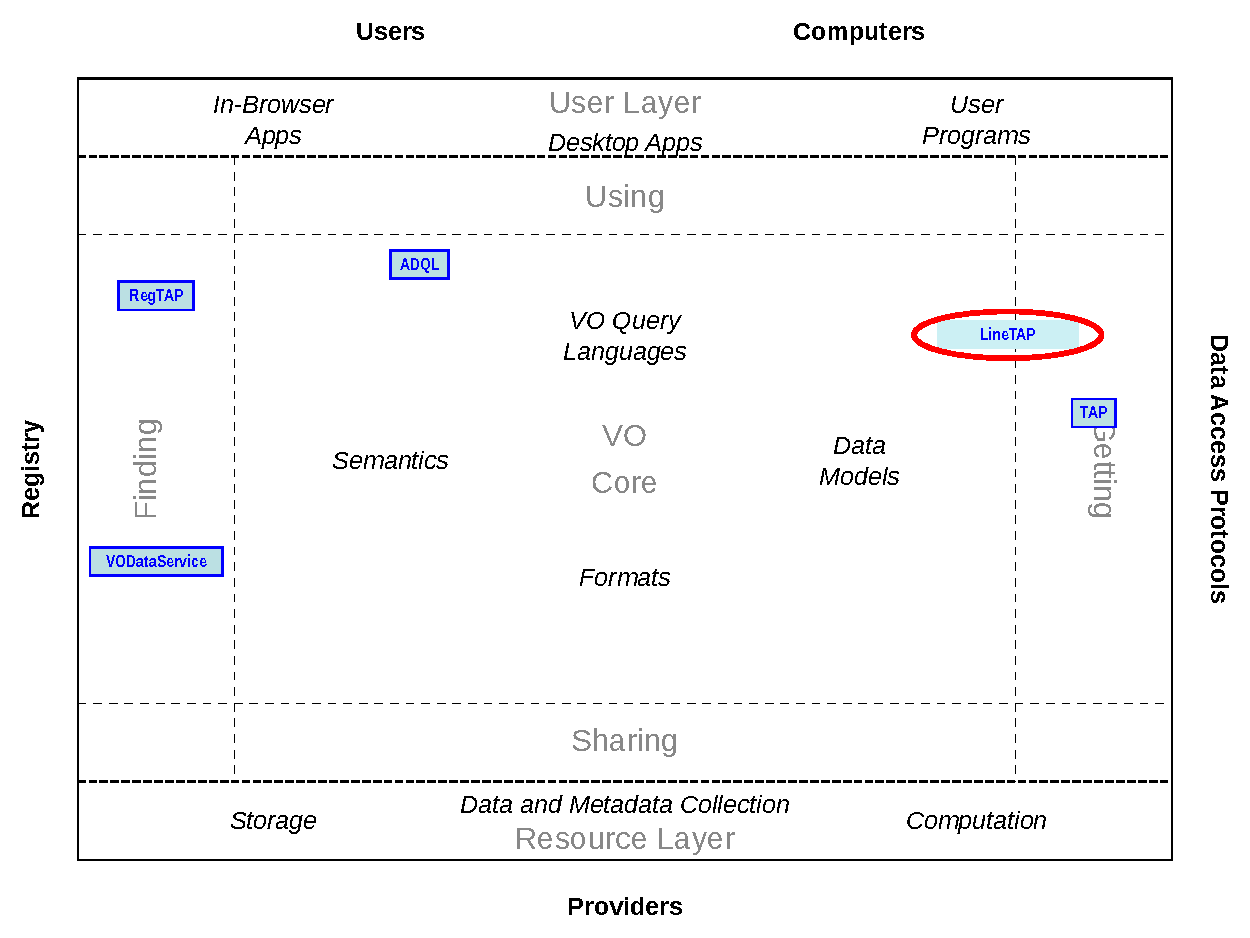
\includegraphics[width=0.9\textwidth]{role_diagram.pdf}
\caption{Architecture diagram for LineTAP}
\label{fig:archdiag}
\end{figure}

Fig.~\ref{fig:archdiag} shows the role this document plays within the
IVOA architecture \citep{2021ivoa.spec.1101D}.  It is using TAP
\citep{2019ivoa.spec.0927D} for the communication of queries to the
server and the results back to the client, where the queries are written
in ADQL \citep{2008ivoa.spec.1030O}.  To make LineTAP tables
discoverable, they are registered using VODataService's
\citep{2021ivoa.spec.1102D} tablesets, and we give recipes on how to
discover them using RegTAP \citep{2019ivoa.spec.1011D}.


\section{Use Cases}
\label{sect:use-cases}

LineTAP really only has a single use case, the discovery of spectral
lines for identification purposes.  To structure standards development,
we discuss some situations specifically:

\subsection{Identifying a Single Line}

A user sees a feature in a spectrum with known (and realiable) spectral
calibration and now wants to know what might possibly be responsible for
it.  Hence, they query a narrow spectral range and retrieve all known
lines from all services.

To select which of the candidate lines are plausible matches, users
would inspect line metadata such as the originating atom or molecule, the
ionisation state, and perhaps oscillator strengths.

\subsection{Getting Properties of Well-Known Lines}

A user wants to display, say, the Lyman series over a plot of a
spectrum.  Hence, a client needs to discover which service holds such
data, select the appropriate records -- presumably by their properties,
perhaps even by their name --, and retrieve them.  If multiple services
hold the desired data, it might need to reconcile differing
specifications.


\subsection{Retrieving Spectral Lines for Cross-Identification}

Users may have various reasons to retrieve a larger number of spectral
lines:

\begin{itemize}
\item When analysing a given spectrum, selecting spectral lines that may
fit the ones in the spectrum, for instance to establish the source's
chemistry or physical state.  Depending on the prior knowledge of the
source, they will want to constrain the matches to specific species in
specific ionisation (or even excitation) states.

\item When estimating the redshift of an object, features found in the
spectrum need to be matched to the rest wavelengths.

\item When computing theoretical spectra, a comparison to the (observed)
ground truth is desirable.
\end{itemize}

The challenge in all these cases is that displaying all lines
known obviously is impossible due to the sheer volume of the data,
and it would not help users in any way.
Hence, the client needs to have some idea of which lines can be expected
to be strong given the physics of the emission's source region.

Selecting the lines before retrieval is a significant optimisation in
this case, as in wider spectra at least hundreds of thousands of lines
will be within the spectral range, while it probably rarely makes sense
to plot more than a hundred or so.  Hence, careful selection of lines
can reduce the volume of data transferred and processed by the client by
several orders of magnitude.

To make good on this promise, the tables need to be queryable such that
lines suspected to be strong for some combination of chemistry,
temperature, and pressure can be filtered out with some accuracy.


\subsection{Finding spectral lines for specific species}

Using a mass spectrometer, researchers find a molecule with the
sum formula C$_{16}$H$_{10}$  in a comet particle.  They now want to
figure out whether any line in the spectrum of the coma of the parent
object corresponds to some molecule with that sum formula.
Conversely, a researcher may want to find lines of Methane or perhaps
even Methane with one hydrogen atom being replaced by a deuteron.


\subsection{Credit}

In particular to provide an incentive to contribute to the global
repository of line data, it should be as simple as possible for users to
give credit to the contributors of line data.


\subsection{Non-Use Cases}

This specification differs from VAMDC in that it does not attempt to
cover all possible uses of spectral line data.  In particular, no
attempt is made to

\begin{itemize}
\item Publish sufficient information to feed sophisticated,
high-precision atmosphere models.
\item Deal with solid-state spectroscopy.
\item Publish lines of non-electromagnetic messengers.
\end{itemize}


\begin{table}[hpt]
\hskip -0.05\linewidth
\begin{tabular}{p{0.43\linewidth}cp{0.5\linewidth}}
\sptablerule
\textbf{Name [Unit]} \ucd{UCD}&\textbf{Type}&\textbf{Description}\\
\sptablerule
% GENERATED: python3 make-columns-table.py
\texttt{title} \hfil\break\ucd{meta.id} & \textbf{text} & \raggedright Human-readable line designation.\tabularnewline
\rowsep
\texttt{vacuum\_wavelength} [Å] \hfil\break\ucd{em.wl} & \textbf{float} & \raggedright Vacuum wavelength of the transition\tabularnewline
\rowsep
\texttt{vacuum\_wavelength\_error} [Å] \hfil\break\ucd{stat.error;em.wl} & float & \raggedright Total error in vacuum\_wavelength\tabularnewline
\rowsep
\texttt{method} \hfil\break\ucd{meta.code.class} & text & \raggedright Method the wavelength was obtained with (XSAMS controlled vocabulary)\tabularnewline
\rowsep
\texttt{element} \hfil\break\ucd{phys.atmol.element} & text & \raggedright Element name for atomic transitions, NULL otherwise.\tabularnewline
\rowsep
\texttt{ion\_charge} \hfil\break\ucd{phys.electCharge} & integer & \raggedright Total charge (ionisation level) of the emitting particle.\tabularnewline
\rowsep
\texttt{mass\_number} \hfil\break\ucd{phys.atmol.weight} & integer & \raggedright Number of nucleons in the atom or molecule\tabularnewline
\rowsep
\texttt{upper\_energy} [J] \hfil\break\ucd{phys.energy;phys.atmol.initial} & float & \raggedright Energy of the upper state\tabularnewline
\rowsep
\texttt{lower\_energy} [J] \hfil\break\ucd{phys.energy;phys.atmol.final} & float & \raggedright Energy of the lower state\tabularnewline
\rowsep
\texttt{inchi} \hfil\break\ucd{meta.id;phys.atmol;meta.main} & text & \raggedright International Chemical Identifier InChI.\tabularnewline
\rowsep
\texttt{inchikey} \hfil\break\ucd{meta.id;phys.atmol} & text & \raggedright The InChi key (hash) generated from inchi.\tabularnewline
\rowsep
\texttt{einstein\_a} \hfil\break\ucd{phys.atmol.transProb} & float & \raggedright Einstein A coefficient of the radiative transition.\tabularnewline
\rowsep
\texttt{xsams\_uri} \hfil\break\ucd{meta.ref} & text & \raggedright A URI for a full XSAMS description of this line.\tabularnewline
\rowsep
\texttt{line\_reference} \hfil\break\ucd{meta.ref} & text & \raggedright Reference to the source of the line data; this could be a bibcode, a DOI, or a plain URI.\tabularnewline

% /GENERATED
\sptablerule
\end{tabular}
\caption{The columns that make up the LineTAP data model.  Column names
and units are mandatory, columns with types in \textbf{bold face} must
not be NULL.}
\label{tab:ltcols}
\end{table}


\section{Spectral Line Data}\label{sect:quantities}

Table~\ref{tab:ltcols} gives the columns that make up the LineTAP
relational model.  Implementations MUST have all columns given in this
table, MUST exactly declare the units as given there, and MUST NOT have
NULL values in columns with types printed in bold face in the table.
Implementations are free to adapt the UCDs and descriptions given in the
table, but they SHOULD give UCDs and descriptions for all columns.

Column types can be adjusted to local needs; in the
above table, ``float'' is to be understood as any suitable
floating-point number, ``integer'' as any integral type, and ``string''
some sort of character sequence.

Implementors are free to add additional, custom columns.

Implementors wishing to communicate the quantum numbers of the two
states participating in the transition SHOULD use the column names
\textit{lo\-wer\_sta\-te\_configuration} and
\textit{up\-per\_sta\-te\_configuration}.  This specification does not
constrain the content of these columns, and hence these cannot be
queried or interpreted interoperably.

The following additional notes apply to individual columns:

\begin{itemize}

\item \texttt{title} This is a human readable string representing the
element or molecule producing the line.  Implementors are free to choose
titles as they see it, but they should keep in mind that these titles
should work in cramped places (i.e., they should not exceed 20
characters or so) and that they should speak to astronomers.  ``21 cm
HI'' or ``[NII]6583'' would be good examples.

\item \texttt{vacuum\_wavelength}
All wavelengths in LineTAP are given for the vacuum,
and  they are stored in the database in
Angstrom.  An  ADQL user-defined function is provided to convert these
wavelengths to other units. They will be described in
sect.~\ref{sect:udfs}.

\item \texttt{vacuum\_wavelength\_error} The integrated error for the
\texttt{vacuum\_wave\-length}.  This subsumes the complex error model of
VAMDC and is obviously not intended to replace it for precise analyses.
Data providers should, where necessary, combine systematic and
statistical errors.  Where the original errors are asymmetric, this
quantity should ideally reflect the FWHM of a Gaussian fit of the true
error profile, or simply employ the larger error as an upper limit.

\item \texttt{method} Describes which method was used to obtain the
wavelength value. The method names admitted here are listed in the XSAMS
Schema\footnote{\url{https://standards.vamdc.eu/dataModel/vamdcxsams/methods.html\#method}}.

\item \texttt{element} For atomic lines, this column gives the
conventional IUPAC element symbol (e.g., H, He, or Rn), using the
conventional capitalisation (i.e., uppercase first letter, lowercase
second letter where present).  No additional qualifications are admitted
here; use \texttt{ion\_charge} to denote ionisation levels and
\texttt{mass\_number} to distinguish isotopes.  Molecular transitions
have NULL here; use \texttt{inchi} and \texttt{inchikey} to identify
those.  For atomic transitions, \texttt{element} is mandatory.

\item \texttt{ion\_charge} Ionization level of the species.

\item \texttt{mass\_number} The mass number of an atom or the sum of
each atomic mass numbers of the elements forming a molecule.

\item \texttt{upper\_energy} Energy  in J of the quantum state
with higher energy

\item \texttt{lower\_energy} Energy  in J of the quantum state
with lower energy

\item \texttt{inchi} The IUPAC International Chemical Identifier
(InChI), which  provides unique labels for well-defined chemical
substances \citep{INCHI}. It is meant to be human readable, but
depending of the molecule it can be very long.  Here, the main layer is
mandatory, the charge, stereochemical, and isotopic layers are optional.
Only standard InChIs may be used in LineTAP.  This is optional for
atomic transitions (hence, query using \texttt{element},
\texttt{ion\_charge}, and \texttt{mass\_number} for those) but mandatory
for molecules.

\item \texttt{inchikey} Character signature based on a hash code of
the InChI string. It will be used to uniquely identify species.  As with
\texttt{inchi}, this is optional for atomic transitions but mandatory
for molecules.

\item \texttt{einstein\_a} Einstein coefficient, or transition probability.

\item \texttt{xsams\_uri} Where full XSAMS metadata is available for a
transition, this link resolves to that document. What is returned MUST
return exactly one transition, and it MUST be in XSAMS version 1.

\item \texttt{line\_reference} Information about the source of the line data,
like an URI, DOI or bibcode.

\end{itemize}


\section{Protocol}
\label{sect:protocol}
\subsection{Queries: LineTAP}

\subsection{User-defined functions}
\label{sect:udfs}

LineTAP services MUST implement the \texttt{ivo\_specconv} user defined
function as defined by the Catalogue of ADQL User Defined Functions
\citep{2021ivoa.spec.0310C}\todo{Update to a reference to 1.1 when it is
actually in}.

With this function, users can query LineTAP databases in their preferred
units, as in

\begin{lstlisting}[language=SQL]
SELECT
  title,
  ivo_specconv(vacuum_wavelength, 'GHz') as freq
WHERE
  vacuum_wavelength BETWEEN ivo_specconv(200, 'GHz', 'Angstrom')
    AND ivo_specconv(300, 'GHz', 'Angstrom')
\end{lstlisting}

The shorter alternative

\begin{lstlisting}[language=SQL]
SELECT
  title,
  ivo_specconv(vacuum_wavelength, 'GHz') as freq,
WHERE
  ivo_specconv(vacuum_wavelength, 'GHz') BETWEEN 200 AND 300
\end{lstlisting}

\noindent would work as well but will probably put a significantly higher load on
the server machine.  It is therefore discouraged.

Also note that since unit conversions may be non-linear, it is generally
wrong to use \texttt{ivo\_specconv} on
\texttt{vacuum\_wavelength\_error}.


\section{LineTAP Query Examples}

\subsection{Use Case Examples}

In this section, we give queries addressing the use cases from
section~\ref{sect:use-cases}.

\subsubsection{Identifying a Single Line}

To obtain human-readable labels for a feature between 4005 and 4005.5
Angstrom, run:

% please-run-a-test
\begin{lstlisting}[language=SQL]
SELECT title, vacuum_wavelength
FROM toss.line_tap
WHERE
  vacuum_wavelength BETWEEN 4005 AND 4005.5
\end{lstlisting}

While we suggest it is in general preferable to do unit conversion
client-side, here is how to express such a query in
frequency.
Note that you will have to swap lower and upper limits when converting
from energy or frequency to wavelength.

%please-run-a-test
\begin{lstlisting}[language=SQL]
SELECT title, ivo_specconv(vacuum_wavelength, 'THz')
FROM toss.line_tap
WHERE
  vacuum_wavelength BETWEEN
    ivo_specconv(6.01, 'THz', 'Angstrom')
    AND ivo_specconv(6.00, 'THz', 'Angstrom')
\end{lstlisting}


\subsubsection{Retrieving Atomic Spectral Lines for Identification}

When a researcher has reason to believe significant amounts of
Technetium are in a hot atmosphere, a client might look for lines for
three and four times ionised Technetium between 3000 and
3500 Angstrom using the element column:

%please-run-a-test
\begin{lstlisting}[language=SQL]
SELECT *
FROM toss.line_tap
WHERE
  element = 'Tc'
  AND ion_charge BETWEEN -4 AND -3
  AND vacuum_wavelength BETWEEN 3000 AND 3100
\end{lstlisting}


\subsubsection{Finding Molecular Spectral Lines for Specific Species}

Where species are only known by elemental composition, lines can be
located using SQL patterns against the inchi column, for instance:

% please-run-a-test
\begin{lstlisting}[language=SQL]
SELECT *
FROM casa_lines.line_tap
WHERE
  inchi LIKE 'InChI=1S/C4H3N/%'
\end{lstlisting}

For a well-defined species, clients should use the InChi key to
constrain the species.  For
normal water, that would be:

% please-run-a-test
\begin{lstlisting}[language=SQL]
SELECT title, vacuum_wavelength, method, einstein_a
FROM casa_lines.line_tap
WHERE
  inchikey='XLYOFNOQVPJJNP-NJFSPNSNSA-N'
\end{lstlisting}

\noindent -- for water with one Hydrogen substituted
with Deuterium, the InChI key
would be XLYOFNOQVPJJNP-DYCDLGHINA-N.

\subsubsection{Selecting Candidate Lines}

To only retrieve the 10 lines with the highest Einstein A for a given
species (in this case, CN) and having an upper level in the octave
around
$1.5\,\textrm{meV}$ above the ground state, one would write

% please-run-a-test
\begin{lstlisting}[language=SQL]
SELECT TOP 10
  title, vacuum_wavelength, einstein_a, line_reference,
  ivo_specconv(upper_energy, 'J', 'eV') as ue, inchi
FROM casa_lines.line_tap
WHERE
  inchikey='JEVCWSUVFOYBFI-UHFFFAOYSA-N'
  and upper_energy between
    ivo_specconv(1, 'meV', 'J')
    AND ivo_specconv(2, 'meV', 'J')
ORDER BY einstein_a DESC
\end{lstlisting}


\subsubsection{Characterising a Service's Data Holdings}

Determining how many lines of which species are available on a given
service could be done with a query like this:

% please-run-a-test
\begin{lstlisting}[language=SQL]
SELECT
  inchi, count(*) as n_lines
FROM casa_lines.line_tap
GROUP BY inchi
\end{lstlisting}

\section{Mapping from VAMDCXSAMS}
\label{sect:mapping}

The quantities used in the mapping belong to the following elements of XSAMS
Schema\footnote{\url{https://vamdc.org/documents/vamdc-xsams-doc-1.0/}\label{fn:schema}}.

\begin{itemize}
\item \xsref{XSAMSData.Species.Atoms.Atom}
\footnote{\url{https://standards.vamdc.eu/dataModel/vamdcxsams/speciesAtoms.html\#atom}\label{fn:atom}},
\item \xsref{XSAMSData.Species.Molecules.Molecule}
\footnote{\url{https://standards.vamdc.eu/dataModel/vamdcxsams/speciesMolecules.html\#molecule}\label{fn:molecule}},
\item \xsref{XSAMSData.Processes.Radiative.RadiativeTransition}
\footnote{\url{https://standards.vamdc.eu/dataModel/vamdcxsams/processRadiative.html\#radiativetransition}\label{fn:radtrans}},
\item \xsref{XSAMSData.Sources}
\footnote{\url{https://standards.vamdc.eu/dataModel/vamdcxsams/sources.html}\label{fn:source}}
\end{itemize}

Listed below are the LineTAP quantities defined in section \ref{sect:quantities} and the corresponding elements from the XSAMS schema:

\begin{bigdescription}
\item [vacuum\_wavelength]
  \begin{xsamsbridge}
  \item[data model] \xsref{RadiativeTransition.EnergyWavelength}\xsamsref{fn:radtrans}
  \item[constraints] if \xsref{vacuum} is not true, use
    \xsref{AirToVac} to convert.
  \end{xsamsbridge}

\item [vacuuml\_wavelength\_error]
  \begin{xsamsbridge}
   \item[data model] \xsref{RadiativeTransition.EnergyWavelength}, \xsref{DataType.Accuracy} \footnote{%
  \url{https://standards.vamdc.eu/dataModel/vamdcxsams/types.html\#accuracytype}}

  \end{xsamsbridge}

\item [method]
 \begin{xsamsbridge}
  \item[data model] \xsref{RadiativeTransition.EnergyWavelength.Method}
     \xsamsref{fn:radtrans} \footnote{\url{https://standards.vamdc.eu/dataModel/vamdcxsams/methods.html\#method}}
 \item[constraints]
    \xsref{MethodID} must be equal to
    \xsref{MethodRef} of the respective energy wavelength. Possible values are given in the VAMDC standard.
   \end{xsamsbridge}

\item [inchi]
  \begin{xsamsbridge}
  \item[data model] \xsref{Atom.Isotope.Ion.InChi}
    \footnote{\url{https://standards.vamdc.eu/dataModel/vamdcxsams/speciesAtoms.html\#atomicion}\label{fn:ion}} or
    \xsref{Molecule.MolecularChemicalSpecies.InChI}
    \footnote{\url{https://standards.vamdc.eu/dataModel/vamdcxsams/speciesMolecules.html\#molecularchemicalspecies}\label{fn:moleculespecies}}
  \item[constraints]
    \xsref{SpeciesRef} of radiative transition must be equal
      to \xsref{SpeciesID} of  the respective atom or molecule.

  \end{xsamsbridge}

\item [inchikey]
  \begin{xsamsbridge}
    \item[data model] \xsref{Atom.Isotope.Ion.InChiKey}\xsamsref{fn:ion},
      \xsref{Molecule.MolecularChemicalSpecies.InChIKey}\xsamsref{fn:moleculespecies},
    \item[constraints]
      \xsref{SpeciesRef} of radiative transition must be equal
      to \xsref{SpeciesID} of  the respective atom or molecule.
  \end{xsamsbridge}

\item [ion\_charge]
  \begin{xsamsbridge}
    \item[data model] \xsref{Atom.Isotope.Ion.IonCharge}\xsamsref{fn:ion} or
      \xsref{Molecule.MolecularChemicalSpecies.IonCharge}\xsamsref{fn:moleculespecies}

    \item[constraints]
      \xsref{SpeciesRef} of radiative transition must be equal
      to \xsref{SpeciesID} of  the respective atom or molecule.
  \end{xsamsbridge}

\item [mass\_number (atoms)]
  \begin{xsamsbridge}
    \item[data model] \xsref{Atom.Isotope.IsotopeParameters.MassNumber}\xsamsref{fn:atom}

    \item[constraints] \xsref{SpeciesRef} of radiative transition must be equal
      to \xsref{SpeciesID} of  the respective atom or molecule.
  \end{xsamsbridge}

\item [upper\_state\_energy]
  \begin{xsamsbridge}
    \item[data model]
      \xsref{Atom.Isotope.Ion.AtomicState.AtomicNumericalData.StateEnergy}\footnote{\url{https://standards.vamdc.eu/dataModel/vamdcxsams/speciesAtoms.html\#atomicstate}\label{fn:atomicstate}} or
      \xsref{Molecule.MolecularState.MolecularStateCharacterisation.StateEnergy}\footnote{\url{https://standards.vamdc.eu/dataModel/vamdcxsams/speciesMolecules.html\#molecularstate}\label{fn:molecularstate}}
    \item[constraints]
       \xsref{UpperStateRef} must be equal to
    \xsref{StateID}  of the respective molecular state or atomic state.
  \end{xsamsbridge}

\item [lower\_state\_energy]
  \begin{xsamsbridge}
    \item[data model]
      \xsref{Atom.Isotope.Ion.AtomicState.AtomicNumericalData.StateEnergy} \xsamsref{fn:atomicstate} or
      \xsref{Molecule.MolecularState.MolecularStateCharacterisation.StateEnergy}\xsamsref{fn:molecularstate}
    \item[constraints]  \xsref{LowerStateRef} must be equal to
    \xsref{StateID}  of the respective molecular state or atomic state.

  \end{xsamsbridge}

\item [einstein\_a]
  \begin{xsamsbridge}
    \item[data model]
      \xsref{RadiativeTransition.Probability.TransitionProbabilityA} \xsamsref{fn:radtrans}
  \end{xsamsbridge}

\item [line\_reference]
  \begin{xsamsbridge}
    \item[data model] \xsref{Sources.Source.DigitalObjectIdentifier}\xsamsref{fn:source},
      \xsref{Sources.Source.UniformResourceIdentifier}\xsamsref{fn:source}
  \end{xsamsbridge}


\item [title]
      a human readable string for information. Can be composed by the species name  and/or other information that might be useful. This quantity is not part of XSAMS (but part of SSLDM).
\end{bigdescription}

\section{LineTAP and the VO Registry}
\label{sect:regmatters}

\subsection{Registering LineTAP-conforming Tables}

LineTAP tables are registered using VODataService \citep{2021ivoa.spec.1102D}
tablesets, where the table utype is set to
$$\hbox{\verb|ivo://ivoa.net/std/linetap#table-1.0|}.$$

The tableset is normally contained in a VODataService \xmlel{CatalogService}
record with a TAP capability, and this capability normally is an auxiliary
capability as per DDC \citep{2019ivoa.spec.0520D}.  For one-table
services a full TAPRegExt \citep{2012ivoa.spec.0827D} capability is also
allowed; other resource types can be used for registration as
appropriate.

Further capabilities, for instance for full VAMDC or legacy SLAP
services, may be given in the same record.

An example for a registry record in VOResource, for the case of
using an auxiliary capability referencing a main TAP service comes with
this document\footnote{\auxiliaryurl{example-record.xml}}.

The noteworthy points in the record are:

\begin{itemize}
\item A \xmlel{relationship} element referencing the main TAP service
through which the service is queriable as per DDC:
\begin{lstlisting}[language=XML,basicstyle=\footnotesize]
<relationship>
  <relationshipType>served-by</relationshipType>
  <relatedResource ivo-id="ivo://org.gavo.dc/tap"
    >GAVO Data Center TAP service</relatedResource>
</relationship>
\end{lstlisting}

\item The declaration for the auxiliary capability, including the access
URL so clients do not need to follow the relationship just declared if
all they need is the access URL:
\begin{lstlisting}[language=XML,basicstyle=\footnotesize]
<capability standardID="ivo://ivoa.net/std/TAP#aux">
   <interface role="std" version="1.1" xsi:type="vs:ParamHTTP">
     <accessURL use="base">http://dc.zah.uni-heidelberg.de/tap</accessURL>
   </interface>
</capability>
\end{lstlisting}

\item Most importantly, the declaration of the table utype that lets
clients discover that this particular table contains LineTAP data:
\begin{lstlisting}[language=XML,basicstyle=\footnotesize]
<table>
  <name>toss.ivoa_lines</name>
  <title>TOSS</title>
  <description> The LineTAP version of...</description>
  <utype>ivo://ivoa.net/std/linetap#table-1.0</utype>
  ...
</table>
\end{lstlisting}
\end{itemize}

That in the example record, the resource description is identical to the
description of the schema, which again is identical to the description
of the table is an artefact of LineTAP registrations being single-table
and is thus to be expected in most registrations of this type.  Clients
are advised to use the resource description for full text searches.


\subsection{Discovering LineTAP services}

LineTAP consumers in general are interested in TAP endpoints and table names for
LineTAP services.  By our registration pattern, this translates into
resources with TAP capabilities that have a standard key for version 1
LineTAP in a table utype.

Translated into RegTAP \citep{2019ivoa.spec.1011D}, the following query
would return TAP access URLs and the table names:

\begin{lstlisting}[language=SQL]
SELECT DISTINCT table_name, access_url
FROM rr.res_table
  NATURAL JOIN rr.capability
  NATURAL JOIN rr.interface
WHERE
  table_utype LIKE 'ivo://ivoa.net/std/linetap#table-1.%'
  AND standard_id LIKE 'ivo://ivoa.net/std/tap%'
  AND intf_role='std'
\end{lstlisting}

The \texttt{DISTINCT} in the main query is a rough filter that removes
entries duplicated because their tables are registred both in the main
TAP record and in an auxiliary capability.

The regular expression in the utype match is to make sure minor version
increments do not prevent service discovery; by IVOA versioning rules,
all LineTAP services of minor version 1 can be operated by all LineTAP
clients of version 1.  We do not constrain the version of the TAP
service. Clients may want to adapt the TAP discovery pattern to match
their specific needs.



\appendix
\section{Changes from Previous Versions}

No previous versions yet.
% these would be subsections "Changes from v. WD-..."
% Use itemize environments.


\bibliography{ivoatex/ivoabib,ivoatex/docrepo, localrefs}

\end{document}
